\chapter{Quantitative analysis of Lightning network privacy}

\label{Chapter07LNattacks}

Payment channel networks such as the Lightning Network introduce novel security and privacy challenges.
Multiple attacks on the LN have been described~\cite{Malavolta2017}.
In \textit{value privacy} attacks, the adversary learns payment amounts.
In \textit{relationship anonymity} attacks, the mapping between senders and receivers becomes known.
The \textit{wormhole attack}~\cite{Malavolta2019} allows an adversary to steal fees from honest intermediaries and temporarily block their funds.

In this Chapter, we quantitatively analyze the LN's resistance to the three attacks.\footnote{This Chapter is based on~\cite{Tikhomirov2020a}.}
We estimate attack success probabilities based on a simulated network for an array of parameters.
Our findings suggest that the privacy of the LN depends on highly connected and highly capitalized nodes.
An attacker who successfully compromises those nodes succeeds with a high probability.
Our results are concerned with the LN as described in the specification and apply to all implementations.


\section{Datasets}
\label{sec:datasets}

We use a snapshot of publicly announced LN channels as of 25~February~2020~\cite{fiatjaf2020}.
This snapshot consists of~$5\,929$~nodes and~$35\,233$~channels.
We model the LN as an undirected multi-graph (i.e., may contain multiple edges between each pair of nodes), as two LN nodes can share several channels.
We only consider the largest connected component, which contains $5\,862$~nodes $(98.87\%)$~and~$35\,196$~channels $(99.89\%)$.
We refer to this dataset as \emph{LN20}.\footnote{Our code is available at~\cite{Tikhomirov2019}.}

Based on \emph{LN20}, LN nodes have an average degree of~$12.01$~and a median degree of~$3$~(\cref{fig:node-degree-histogram,fig:channel-capacity-histogram}).
Most nodes have only a few channels, whereas a small number of nodes have many channels.
In particular, $1\,744$~nodes have degree $1$, and the most connected node has $1\,198$~channels.
The capacity is also unequally distributed.
These observations motivate the methodology in our experiments in~\cref{sec:sec-priv-attacks}.

\begin{figure}[tb]
	\centering
	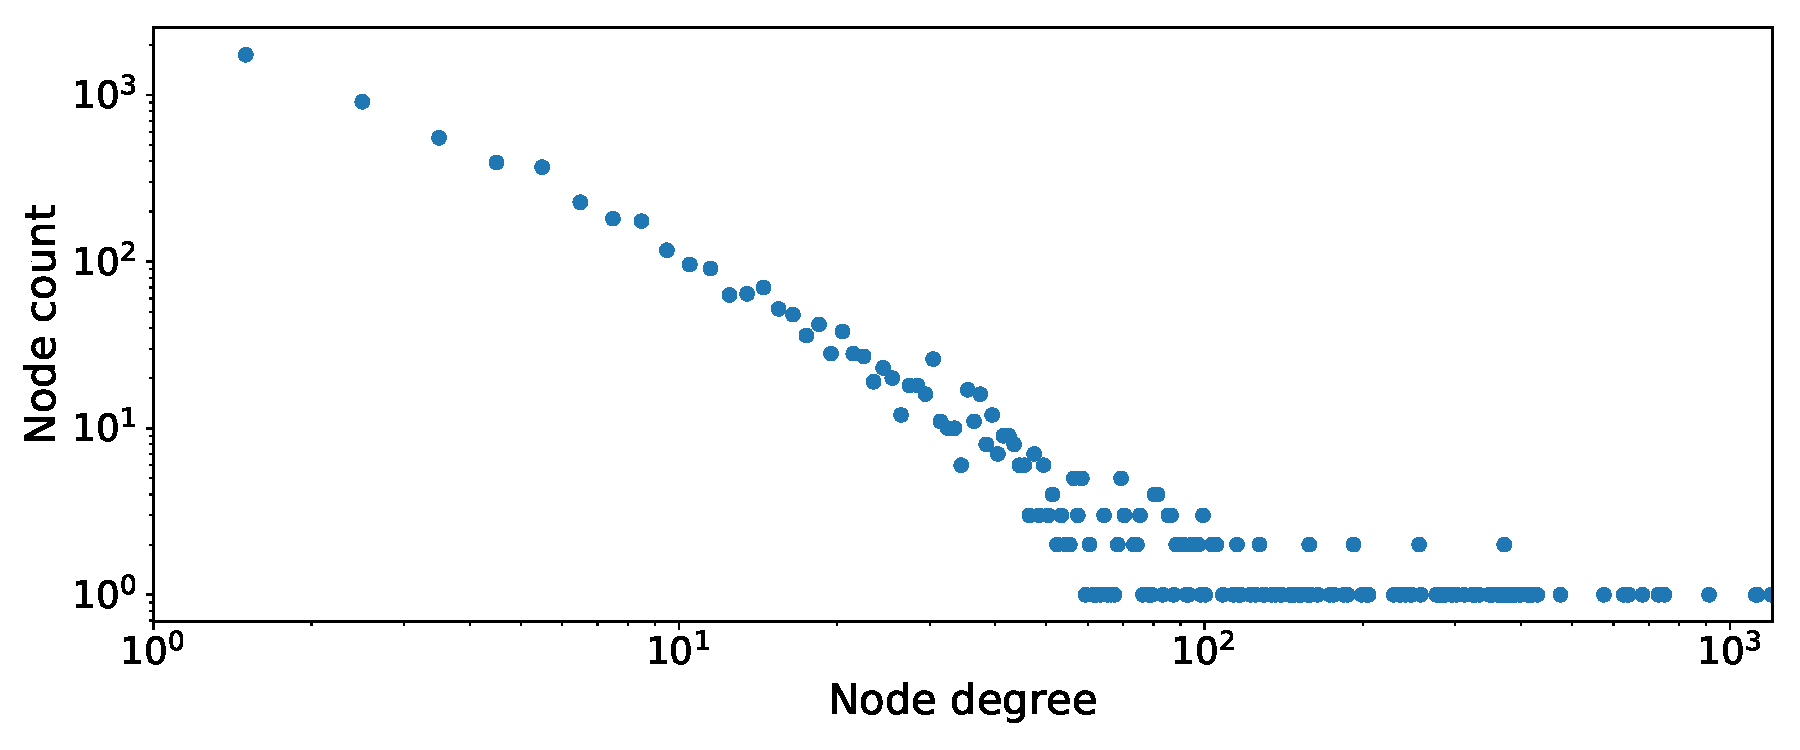
\includegraphics[width=0.8\columnwidth]{node-degree-histogram}
	\caption{Node degree distribution.}
	\label{fig:node-degree-histogram}
\end{figure}

\begin{figure}[tb]
	\centering
	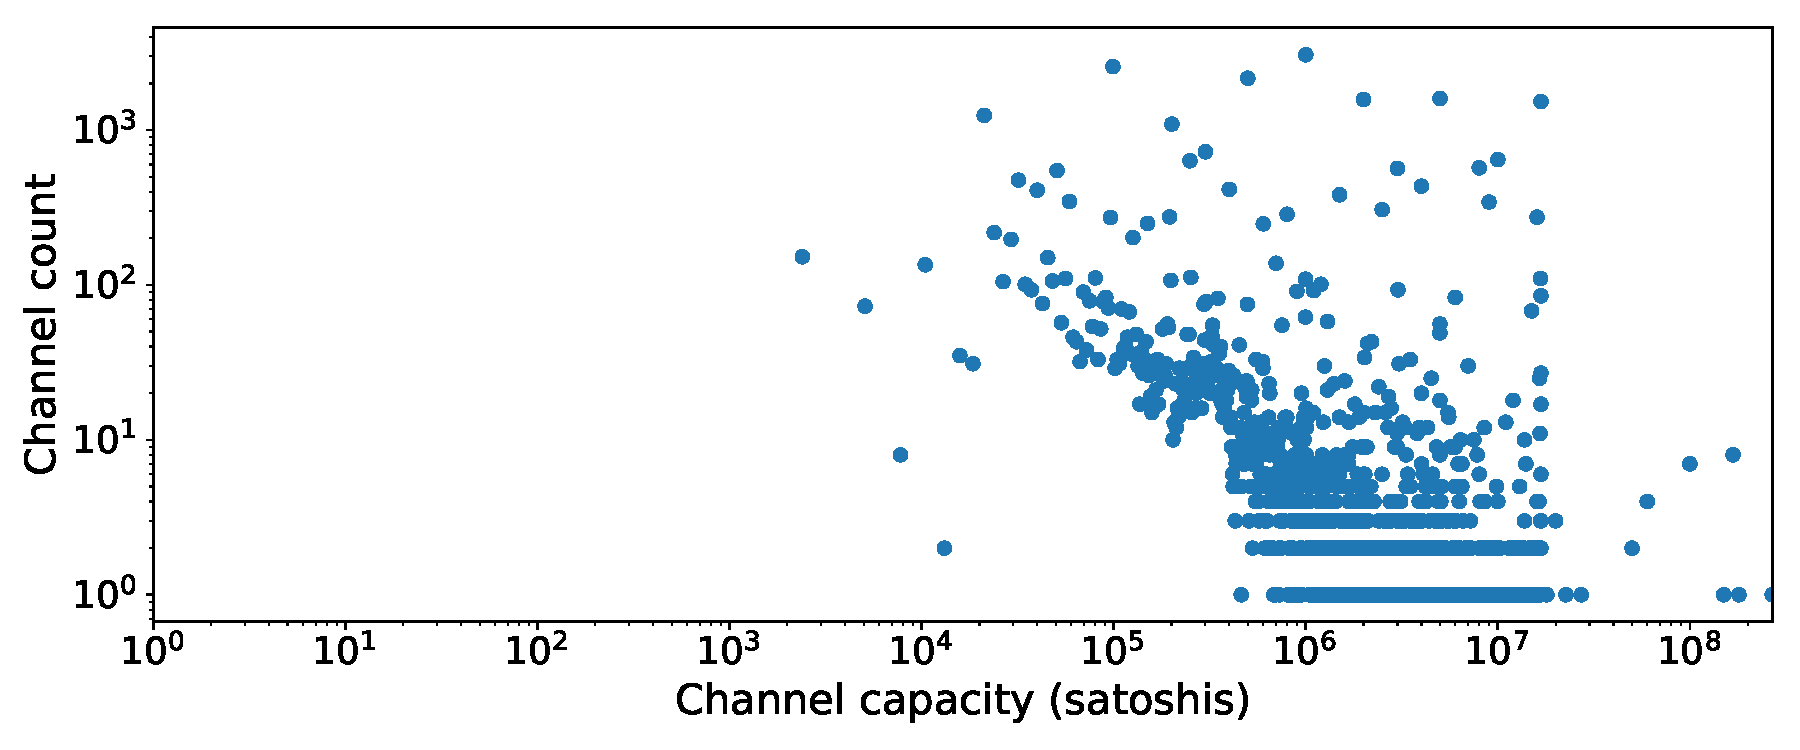
\includegraphics[width=0.8\columnwidth]{channel-capacity-histogram}
	\caption{Channel capacity distribution.}
	\label{fig:channel-capacity-histogram}
\end{figure}

\paragraph{Ethical considerations} 
Our analysis is based solely on publicly available data.
All our calculations use a local representation of the LN network graph obtained from~\cite{fiatjaf2020}.
We do not interfere with the LN activity, nor deanonymize any nodes.


\section{Security and privacy attacks: background}
\label{sec:sec-priv-attacks}

The LN builds upon hash time-locked contracts aiming to achieve atomicity in multi-hop payments.
However,~\cite{Malavolta2019} argues that due to the \emph{wormhole attack}, atomicity does not hold in the LN\@.
Another study~\cite{Malavolta2017} shows that attackers can breach the privacy of LN users.
The feasibility of these attacks depends, among other factors, on the topology of the LN\@.
In this experiment, we aim to quantify the impact of these security and privacy issues on the LN\@.

\begin{figure*}[tb]
	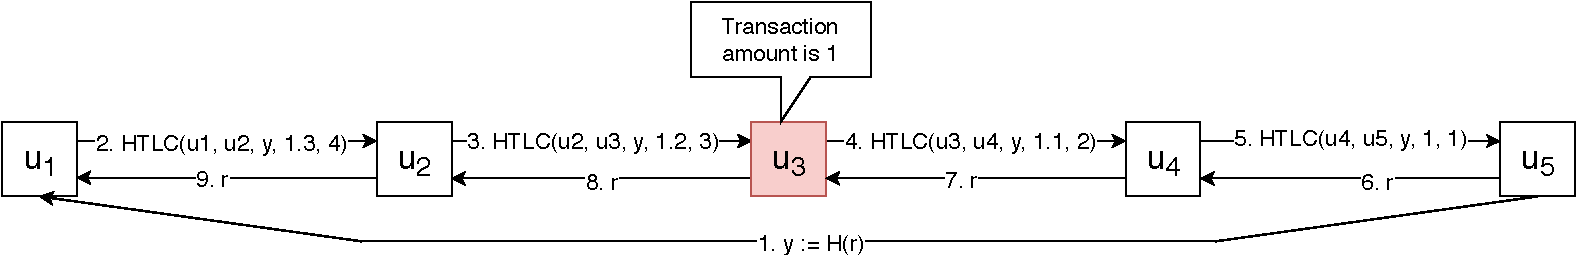
\includegraphics[width=\textwidth]{vp-figure.pdf}
	\vspace{0.3cm}
	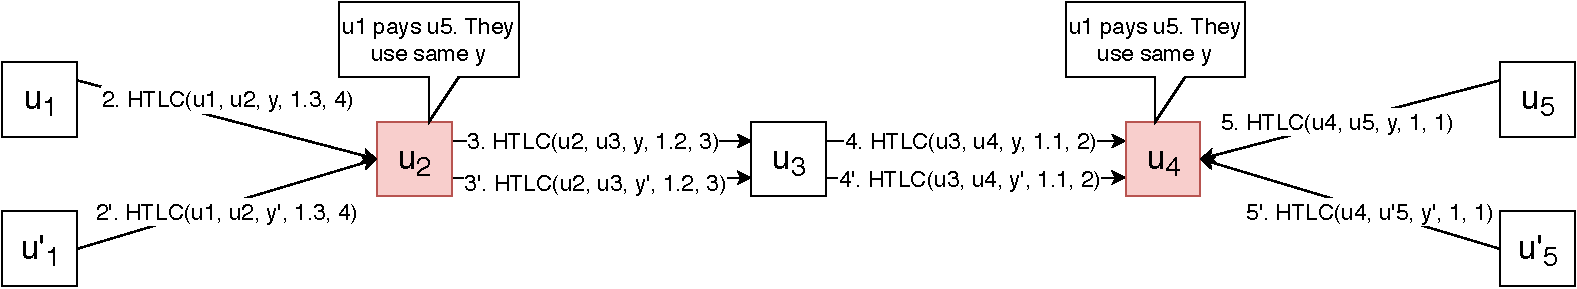
\includegraphics[width=\textwidth]{ra-figure.pdf}
	\vspace{0.3cm}
	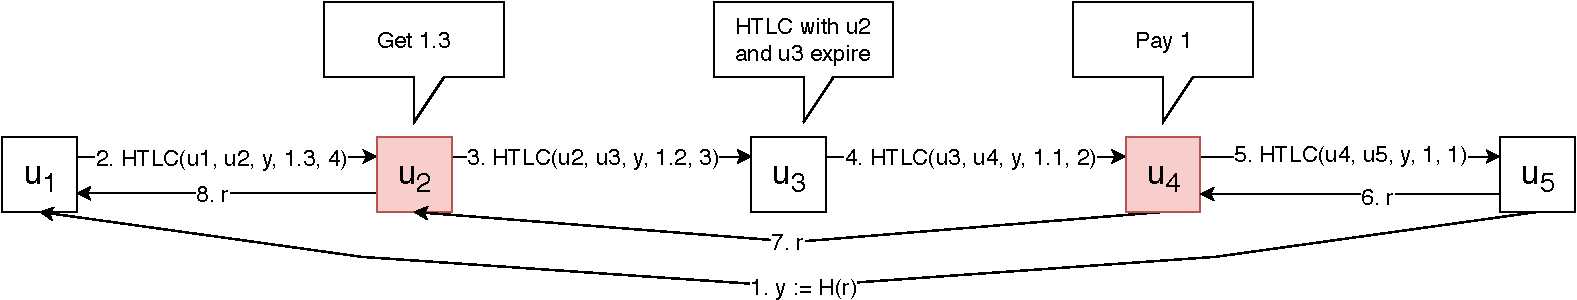
\includegraphics[width=\textwidth]{wa-figure.pdf}
	\caption{An illustrative example of value privacy (top), relationship anonymity (middle), and the wormhole attack (bottom).}
	\label{fig:wormhole-attack}
\end{figure*}

\subsubsection*{Value privacy}
Intuitively, value privacy ensures that for a payment involving only honest users, corrupted users outside the payment path learn no information about the payment value.
This notion thus heavily relies on the existence of paths without malicious nodes.
Otherwise, a malicious intermediary node can trivially learn the (upper bound of the) amount of a payment that it forwards.
For instance, in~\cref{fig:wormhole-attack} the adversary~$u_3$ forwards $1.2$~coins to~$u_4$, estimating the payment amount at around $1$~coin plus forwarding fees.

\subsubsection*{Relationship anonymity}
Intuitively, relationship anonymity ensures that given two simultaneous payments between two pairs of nodes $(u_1, u_2)$ and~$(u'_1, u'_2)$ routed through the same path of intermediary users $i_1, \ldots, i_n$, the adversary controlling some of those intermediaries cannot tell who is paying to whom with probability better than~$1/2$.
However, the LN does not achieve relationship anonymity.
An adversary controlling $i_1$ and~$i_n$ can use the cryptographic challenge included in the HTLC to determine who pays to whom.
For instance, in~\cref{fig:wormhole-attack} the adversary controlling $u_2$ and~$u_4$ can determine that $u_1$ is transacting with~$u_5$ as the same value~$y$ is used along the whole path.
Similarly, $u_2$ and~$u_4$ can determine that $u'_1$ is transacting with~$u'_5$ as the same~$y'$ is used along the path.

\subsubsection*{The wormhole attack}
In the wormhole attack, two colluding nodes in a payment path prevent honest intermediaries from participating in the payment, stealing the fees intended for honest intermediaries.
One may argue that this is not an attack, as, from the sender's point of view, the payment is delivered.
However, this attack diminishes the economic incentive for honest users to forward payments in the first place.

An example of the wormhole attack is depicted in~\cref{fig:wormhole-attack}.
Here, $u_4$ does not send the opening value~$r$ to~$u_3$ (step 7 in~\cref{fig:htlc}).
Instead, $u_4$ sends the value~$r$ to~$u_2$ outside the LN protocol, which allows $u_2$ to settle the HTLC with~$u_1$.
As a result, contracts with~$u_3$ expire, simulating payment failure, and prevent $u_3$ from participating in the payment's successful completion.


\section{Methodology}

We first compute the paths between pairs of nodes.
Given nodes $u_1$ and~$u_2$, we compute the list of paths that connect them with one restriction: we consider only the paths with at most three intermediary nodes.
We observe that these path lengths suffice to allow more than~$85\%$ of payments between a random pair of nodes (\cref{fig:payment-success}) and allow us to exemplify all attacks that we want to study in this experiment.

\begin{figure}
	\centering
	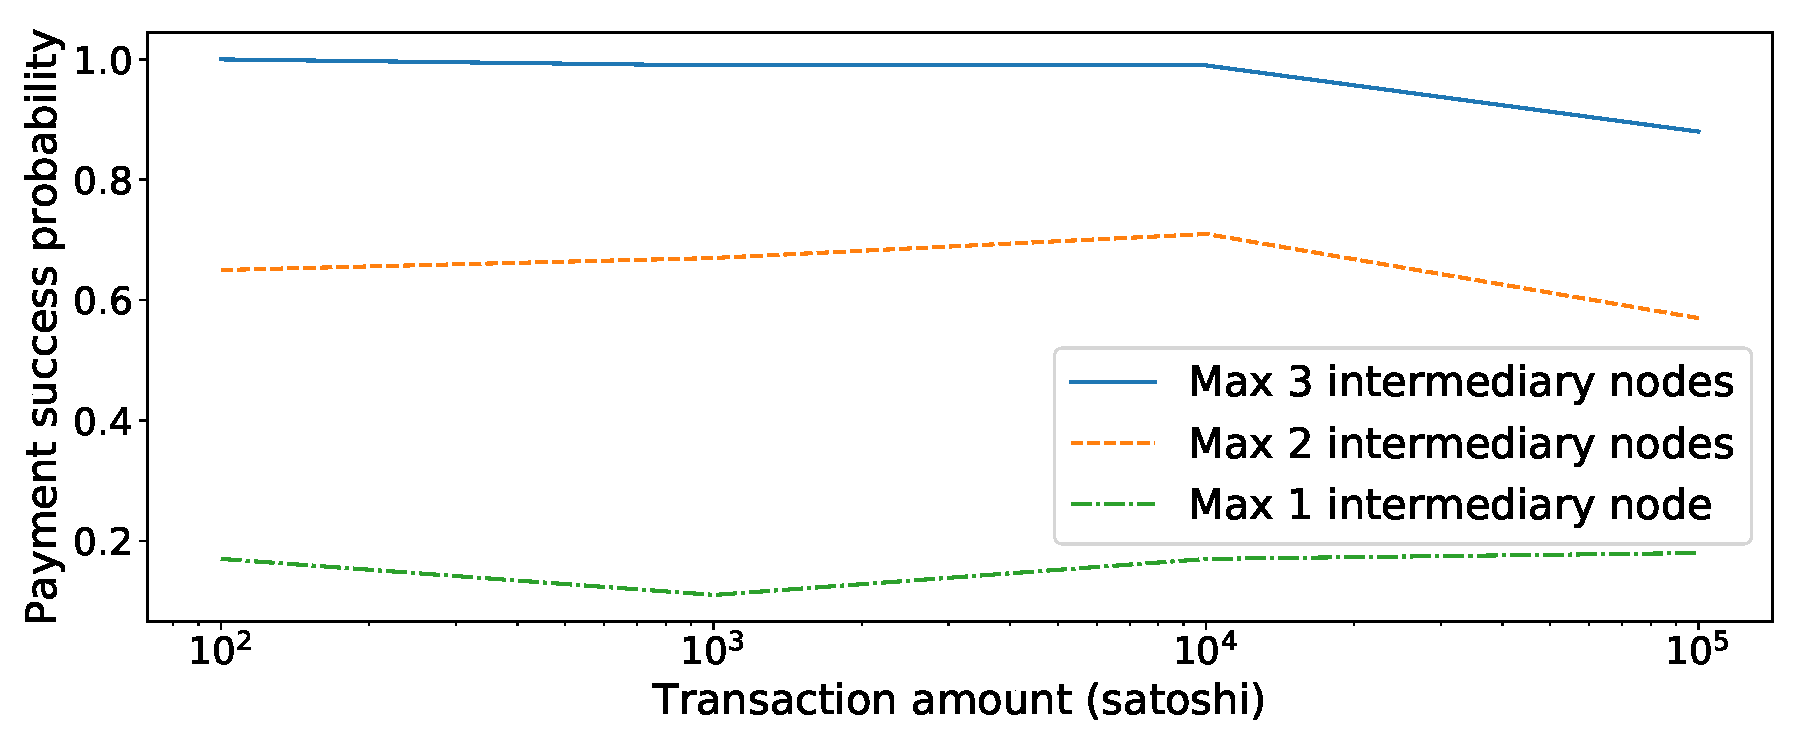
\includegraphics[width=0.8\columnwidth]{payment-success}
	\caption{The share of experiment runs where paths with sufficient capacity exist between sender and receiver.}
	\label{fig:payment-success}
\end{figure}

Let $\textit{paths}_{\langle u_1, u_2 \rangle}$ be the set of paths between $u_1$ and~$u_2$.
We prune the set $\textit{paths}_{\langle u_1, u_2 \rangle}$ into a subset $\textit{paths}_{\langle u_1, u_2 \rangle, x}$, containing only the paths that allow to transfer at least $x$~satoshis.
For instance, $\textit{paths}_{\langle u_1, u_2 \rangle, 10}$ contains the paths between $u_1$ and~$u_2$, which allows transferring at least $10$~satoshis.

For a channel to be capable of transferring $x$~satoshis from~$u_i$ to~$u_j$, $u_i$ must have a balance of at least $x$~satoshis.
However, the current balance of each counterparty in a channel is not publicly available.
Thus, we consider a path suitable for a given payment if the total capacity of every channel in the path is above the payment amount, independently of how this capacity is distributed between the counterparties.
This heuristic might consider a path suitable for a payment while it is not.
We nevertheless follow this heuristic as LN nodes also use it in practice.

As the next step, we study the effectiveness of the selected attack.
For a chosen payment amount~$x$, we split the set $\textit{paths}_{\langle u_1, u_2 \rangle, x}$ into two subsets:

\begin{enumerate}
	\item $\textit{paths-prone}_{\langle u_1, u_2 \rangle, x}$: the subset of paths prone to the attack;
	\item $\textit{paths-safe}_{\langle u_1, u_2 \rangle, x}$: the subset of paths not susceptible to being attacked.
\end{enumerate}

The definition of a path of the form~$u_1 \rightarrow i_1 \rightarrow \ldots \rightarrow i_n \rightarrow u_2$ being prone to the specific attack depends on the attack:

\begin{itemize}
	\item \textit{Value privacy}: We say that a path is prone to the value privacy attack if any intermediary node is under adversarial control.
	
	\item \textit{Relationship anonymity}: We say that a path is prone to the relationship anonymity attack if nodes $i_1$ and~$i_n$ are under adversarial control.
	
	\item \textit{Wormhole attack}: We say that a path is prone to the wormhole attack if there exist two non-neighboring intermediary nodes $i_j$ and~$i_k$  under adversarial control (i.e.,~$j < k$ and~$k \neq j + 1$).
\end{itemize}

Note the difference between the definitions of a prone path in the wormhole attack and the relationship anonymity attack.
The latter does not require an honest user to be located between the two malicious nodes.
For instance, a path of the form $u_1 \rightarrow i_1 \rightarrow i_2 \rightarrow u_2$ where $i_1$ and~$i_2$ are under adversarial control would be considered prone to the relationship anonymity attack but safe against the wormhole attack.

Another aspect that we consider is which nodes are malicious.
We follow three strategies.
First, we assume that nodes with the highest degrees (i.e.,~highly connected nodes) are colluding.
Highly connected nodes have the highest stake in the network.
Thus, an adversary might attempt to corrupt them (e.g.,~by bribery or stealing the private key) to maximize the effect of the attack.
Second, we assume that nodes with the highest total capacity in their adjacent channels are colluding.
Finally, we consider that random nodes are colluding.
We illustrate here that any node (independently of its node degree) might be corrupted.
For instance, the same user might create several LN nodes at strategic positions to carry out the attacks.

We then consider these three attack strategies.
For each number of malicious nodes ($y$) and each strategy, we re-split the set $\textit{paths-prone}_{\langle u_1, u_2 \rangle, x}$ into prone paths and safe paths.
For instance, we denote by $\textit{paths-prone}_{\langle u_1, u_2 \rangle, x, y\textit{-con}}$ the subset of paths between $u_1$ and~$u_2$ that allow to transfer $x$~satoshis and that are prone to the attack if $y$~nodes with the highest node degree are corrupted.
Correspondingly, we denote by $\textit{paths-prone}_{\langle u_1, u_2 \rangle, x, y\textit{-ran}}$ the subset of paths between $u_1$ and~$u_2$ that allow to transfer $x$~satoshis and that are prone to the attack if $y$~nodes chosen uniformly at random are corrupted.

Finally, for each attack strategy, we consider $$\alpha_{\langle u_i, u_j \rangle} := \frac{|\textit{paths-prone}_{\langle u_i, u_j \rangle, x, y}|}{|\textit{paths-prone}_{\langle u_i, u_j \rangle, x, y}| + |\textit{paths-safe}_{\langle u_i, u_j \rangle, x, y}|}$$ the probability that a payment between $u_i$ and~$u_j$ is vulnerable to the attack.
Averaging across all the pairs of nodes tested, we extract the final probabilities reported in~\cref{fig:fig-all-attacks}.

\section{Results and discussion}

\begin{figure*}
	\centering
	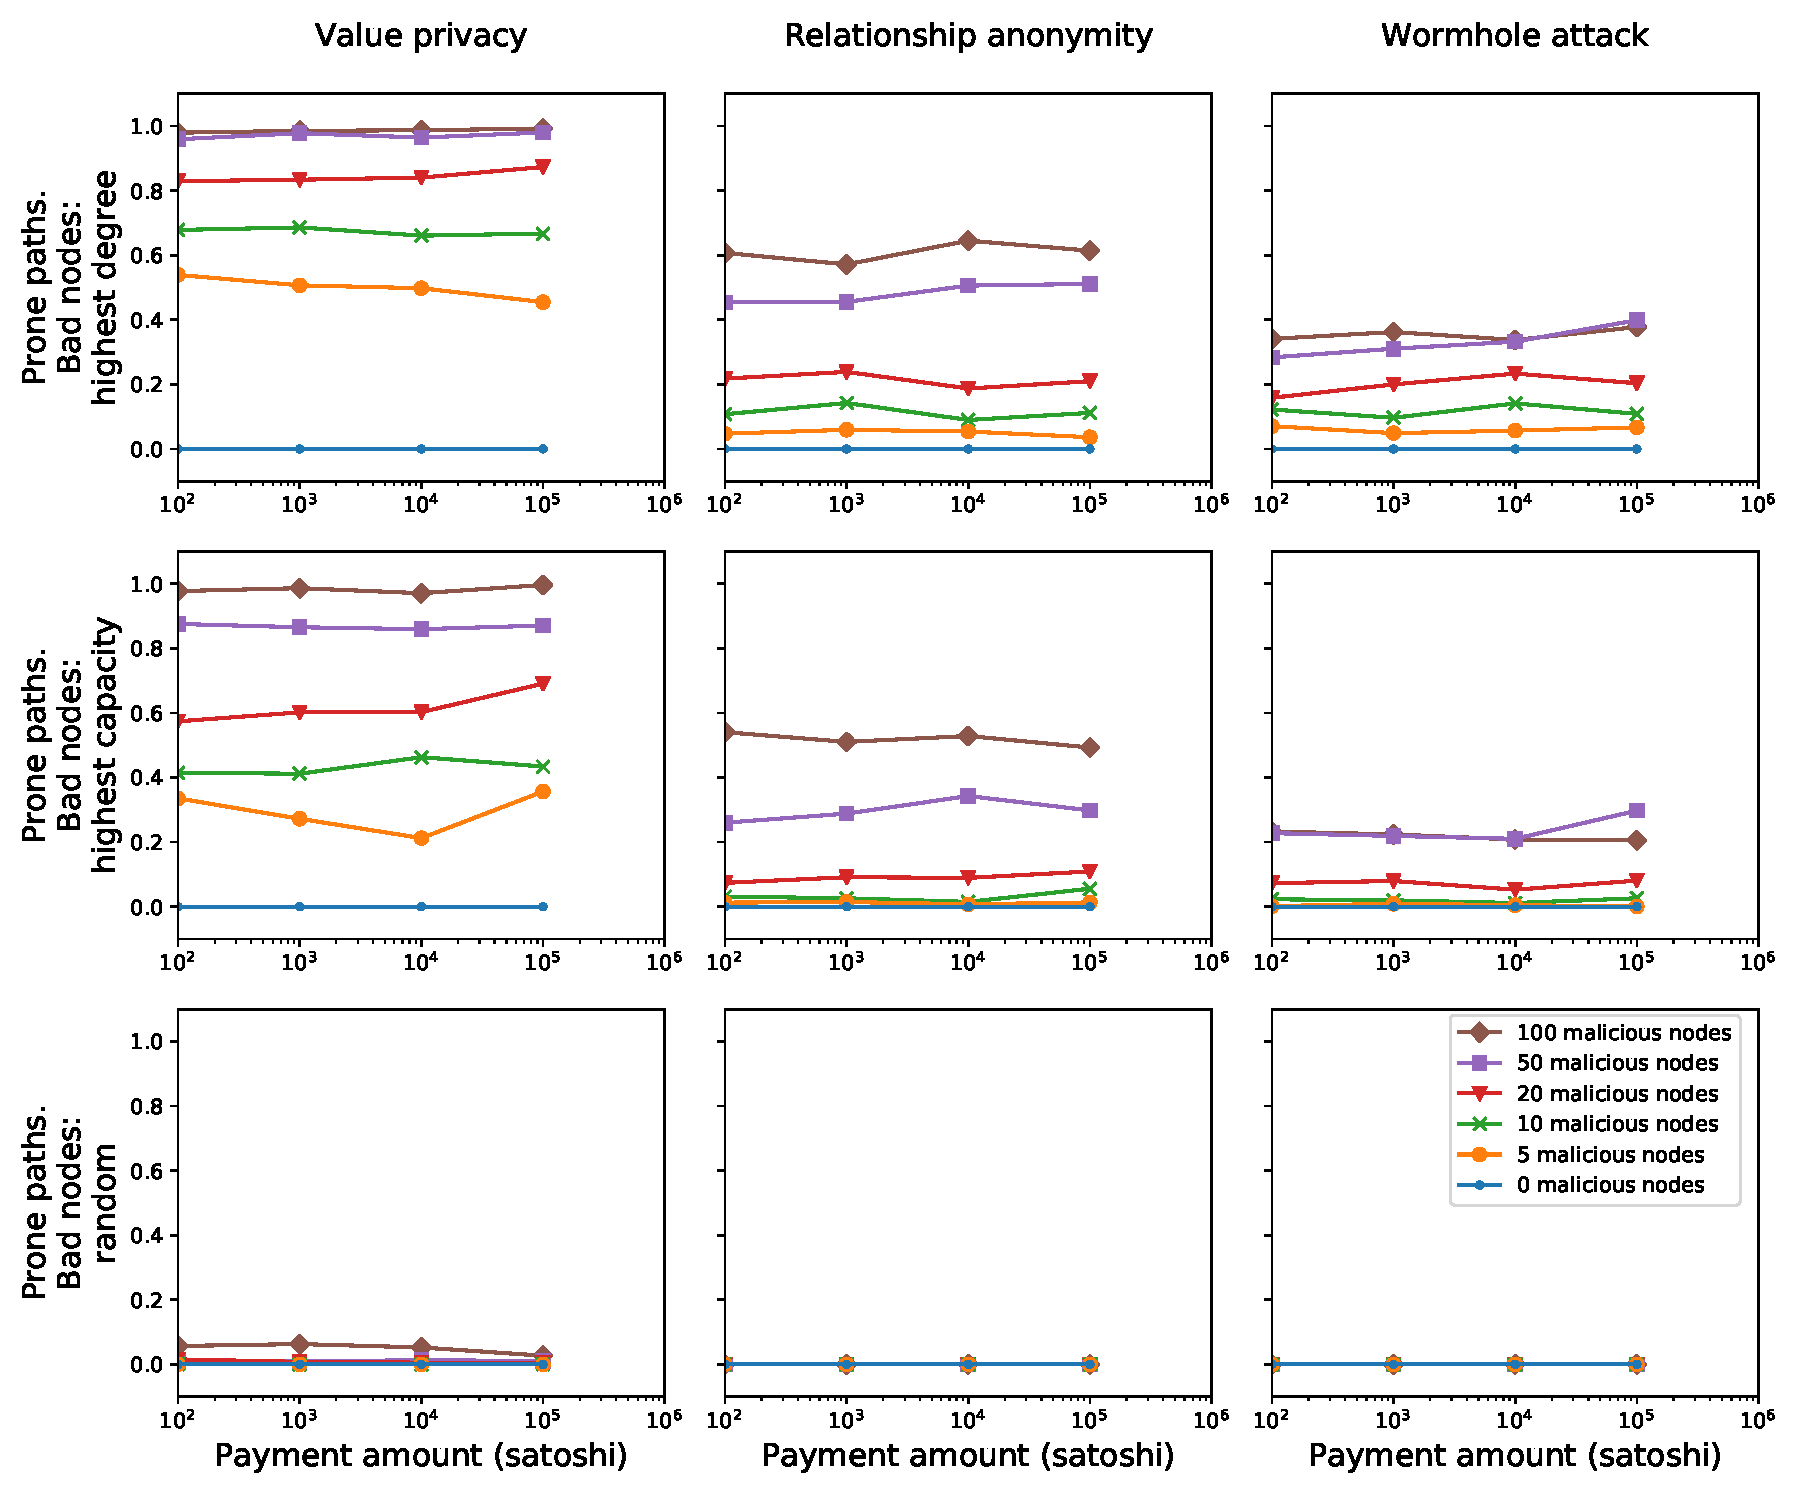
\includegraphics[width=\columnwidth]{fig-all-attacks}
	\caption{Share of prone paths for each parameter combination.}
	\label{fig:fig-all-attacks}
\end{figure*}

For every attack and a given number of compromised nodes, the share of prone paths is relatively stable for all payment amounts (\cref{fig:fig-all-attacks}).
This result indicates that the payment amount does not significantly affect the security of payments.

The three attacks differ in how quickly the share of prone paths changes as the number of compromised nodes increases.
For value privacy, the effect of added highly-connected nodes being compromised is the most profound.
The share of prone paths is $50\%$~if only the $5$~most connected nodes are compromised, and nearly $100\%$~if the $100$~most connected nodes are compromised.
Thus, we conclude that an adversary needs to corrupt only $2\%$~of the nodes to almost nullify any value privacy guarantee in the LN\@.

The average share of prone paths decreases for relationship anonymity.
However, the adversary controlling the $100$~most connected nodes can launch the relationship anonymity attack on about $70\%$~of the paths.
Interestingly, the adversary has fewer possibilities to launch the wormhole attack.
For instance, with~$100$~most connected nodes corrupted, around $30\%$~of the paths are prone to the attack.
A restrictive path structure in the definition of the attack may explain this reduction in the attack's effectiveness.

The attacker benefits less from compromising high-capacity nodes, as opposed to high-degree nodes.
This distinction is most profound for relationship anonymity: around $50\%$ of paths are vulnerable if the~$50$~highest degree nodes are corrupted, but only around~$25\%$~paths are vulnerable if the~$50$~highest capacity nodes are corrupted.
This difference may be explained by the fact that routing algorithms optimize for short paths.
Note that forwarding channels' capacity is not as important as good connectivity, especially for payments of small and medium amounts.

Finally, we consider random nodes compromised.
In contrast to the earlier results, less than $10\%$~of paths are prone to value privacy, and nearly no paths are prone to relationship anonymity and wormhole attacks.
We note that randomly selected nodes have few connections (note the degree distribution in Figure~\ref{fig:node-degree-histogram}).
Thus their compromise does not affect routing at large.

In summary, our results show that highly connected nodes and nodes with high capacity channels have a high impact on the security and privacy of the LN\@.
Assuming that paths are selected uniformly at random from the set of available paths, an adversary that selectively corrupts $100$~(i.e.,~only $2\%$) of LN nodes can effectively learn all the payment values, the sender and the receiver for most payments, and carry out the wormhole attack in about $30\%$~of the paths.
These estimations evidence that the security and privacy attacks shown in theory are indeed crucial in practice.

Carrying out such attacks might be feasible in the live network: an unknown entity under the pseudonym LNBIG is known to control $23$~out of top~$50$~highest connected nodes~\cite{1MLTopConnected} and~$40\%$~of the network capacity~\cite{TheBlockLNBIG} (as of 2019).


\section{Countermeasures}
We assume that every two nodes carry out their payments along a path chosen uniformly at random from the set of all available paths.
However, LN nodes might implement different routing strategies.
For instance, while routing through well-connected nodes improves the chances to reach the receiver through a short and highly liquid path, the sender might instead choose low degree nodes.
Routing around popular nodes may reduce the probability of choosing a compromised path.
We envision a trade-off between connectivity on the one hand and security and privacy on the other, which constitutes a direction for future work.
A node may also route payments through a trusted proxy node, thus guaranteeing that the first node in a path is not compromised.
This strategy would mitigate the relationship anonymity and wormhole attacks (if the path contains no more than three intermediaries).


\section{Conclusion}
\label{sec:conclusions}

The LN has emerged as the most widely deployed solution for scalability issues affecting current blockchains such as Bitcoin.
Despite its conceptual appeal and growing adoption, several works~\cite{Malavolta2017, Malavolta2019} have identified security, anonymity, and scalability limitations.
However, a quantitative analysis of their impact is missing, and this work aims to fill this gap.

We quantitatively study the LN's proneness to the wormhole attack and attacks against value privacy and relationship anonymity.
We observe that a moderately resourceful adversary controlling only $2\%$~of the total node count can carry out these attacks with high success probability.
As the LN evolves, the developers should acknowledge these results in future protocol design decisions.